% status: 10
% chapter: TBD

\title{GraphQL Web APIs}

\author{Averill Cate, Jr}
\orcid{1234-5678-9012}
\affiliation{%
  \institution{The University of Indiana}
  \streetaddress{}
  \city{Bloomington} 
  \state{Indiana} 
  \postcode{47408}
}
\email{acate@iu.edu}

\author{Gregor von Laszewski}
\affiliation{%
  \institution{Indiana University}
  \streetaddress{Smith Research Center}
  \city{Bloomington} 
  \state{IN} 
  \postcode{47408}
  \country{USA}}
\email{laszewski@gmail.com}

% The default list of authors is too long for headers}
\renewcommand{\shortauthors}{A. Cate}

\begin{abstract}
  This project is for Advanced Cloud Computing, Indiana University
  Spring Semester 2018.  Through this project, we will demonstrate the
  use of GraphQL\cite{hid505FacebookGraphQL2018} and cloud computing
  services as a means for constructing and delivering web services.
  The project will rely on The Santa Rita Experimental Range (SRER)
  website and data sets maintained by the Univeristy of Arizona and
  second, related web site, the Walnut Gulch Experimental Watershed
  (WGEW) Online Data Access, maintained by the United States
  Department of Agriculure's, Agriculure Research Service (ARS).
  Neither of these existing sites provide modernized data services,
  yet both sites provide potentiall valuable data to the research
  community.
\end{abstract}

\keywords{hid-sp18-505, GraphQL, Web, Services}

\maketitle

\section{Introduction}
What is GraphQL?  GraphQL is a query language for web application
programer interfaces (APIs)\cite{hid505FacebookGraphQL2018}.  There
have been been many other tools and methods used to develop APIs in
the past.  Some of those older tools are XML and SOAP, JSON and REST,
plain old text or comma separated files.  What makes GraphQL so
different?  First, as the name implies, GraphQL, is a query language.
This is different compared to SOAP/XML and Swagger/REST in that those
tools are a combination of data format and transport protocol.

Typically, SOAP/XML and Swagger/REST APIs are structured so that the
API user needs to review the specifications for interacting with the
API.  For example, what functions or endpoints are available?  What
are the parameters for those functions and what data types apply to
each parameter?  GraphQL is different in that it provides a mechanism
where an API becomes a domain specific language (DSL).  This means
that API consumers can focus on developing transactions with the API
based on the data domain of the API.  For example, a GraphQL API for
stock data would allow API users to format queries something like the
following:

\begin{verbatim}
{
   all_stocks {
     symbol, price, date
}
\end{verbatim}

In this example we see a query request to a GraphQL API that is asking for all 
stock data with respective symbol, price, an date.  Alternatively, a REST based 
query might look like the following:

\begin{verbatim}
http://server.host.com/api/v1/allstocks
\end{verbatim}

In the REST based request we see information related to where the data
are being requested from, the protocol used to make the request, the
API version and finally, what the request is really after, all stock
data.  The latter could be considered more understandble to
programmers or even to someone who is technically a advanced web
users, but compared to the REST request, the GraphQL based request has
a format more closely resembling the data intself and is less concered
with how the data are requested.

A useful way to demonstrate the uses of GraphQL would be to apply
GraphQL to the development of a real-world API that will transform
existing web-based data sources created and maintained at United
Stated Deparment of Agriculture web site and the University of
Arizona.  The first data resource is the Santa Rita Experimental which
is an experimental range currently maintained by the University of
Arizona.  The experimental range was the first of its kind and was
established in 1902\cite{hid505SrerWebSite2018}.  The SRER website, in
its current state, is not structured to deliver data as a service.
The second data source is the Walnut Gulch Experimental Watershed,
which is also an outdoor research facility located in southestern
Arizona\cite{WgewWebSite2018}.  Like the SRER site, the WGEW
preicpitation and runoff data site is not structured to delivered as
services.

\subsection{General Outline}

\begin{enumerate}
\item Web scraping existing data source to download, parse and clean
  existing data.
\item Load the data into a database.
\item Develop a small web application to provide two web services.
  The two services will deliver the same data.  However, one of the
  services will use GraphQL\cite{hid505FacebookGraphQL2018} to deliver
  data and the other will use REST\cite{hid505swaggerio2018} to
  deliver its data.
\item Develop a simple load testing tool that will be used to
  determine performance metrics for both services and compare the
  results of the load tests.
\item Time permitting, create a simple Amazon Lambda service that will
  compute some metric related to the preciption/runoff data.  The
  purpose is to demonstrate how cloud services can be used to off-load
  costs and dependencies on a distributed system like the one proposed
  in this project.
\item Time permitting, develop a 3-node Raspberry Pi cluster to host
  the application.  The purpose of this, is to demonstrate how a
  system like this one can be hosted and deployed on hardware
  infrastructure that is cheap and relatively simple to maintain.
\end{enumerate}

\section{Data Collection}

Data were collected from the Santa Rita Experimental Range website.  In figure 
Figure~\ref{f:srer_landing_page}, we see the present day landing page for SRER.  
What is not apparent in the landing page is the plethora of data available 
data available in the site.

\begin{figure}[htb]
  \centering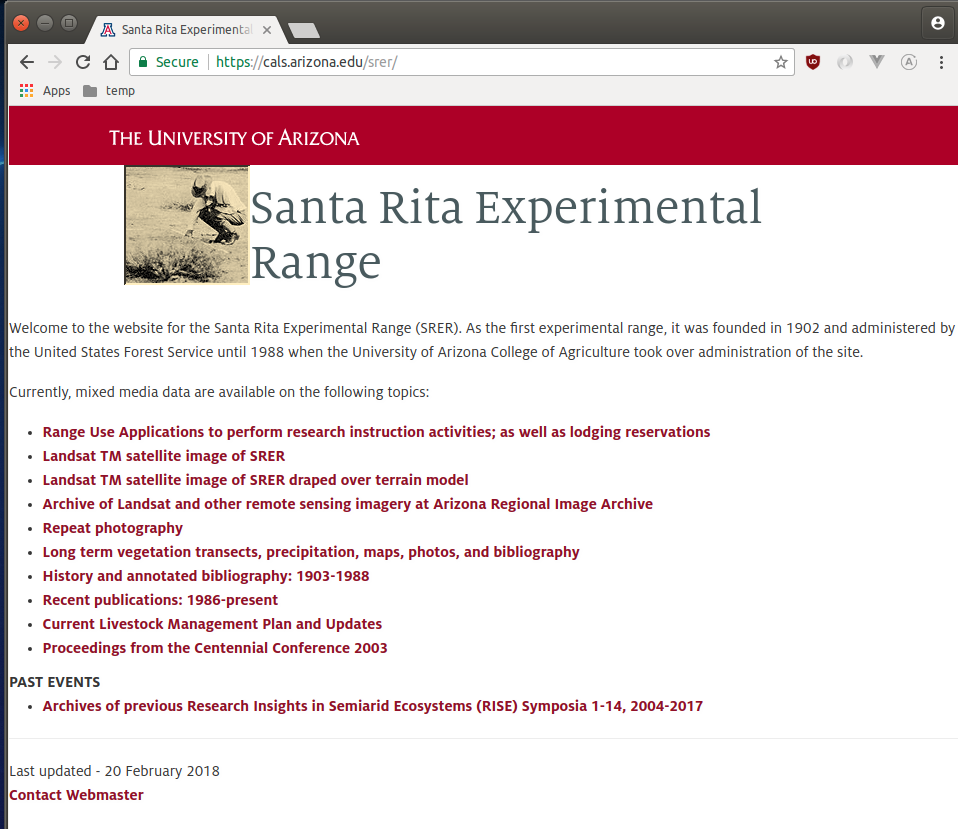
\includegraphics[width=\columnwidth]{./images/srer_landing_page.png}
  \caption{SRER Landing Page \cite{hid505SrerWebSite2018}}\label{f:srer_landing_page}
\end{figure}


In figure~\ref{f:srer_precip_data_page} we have navigated one page deeper into the 
SRER site and as can be seen, meta-data and data are both availabe, but as raw 
text files.  These data are consumable as is, but could be enhanced by being 
made machine readible by creating web services to deliver the data.

\begin{figure}[htb]
  \centering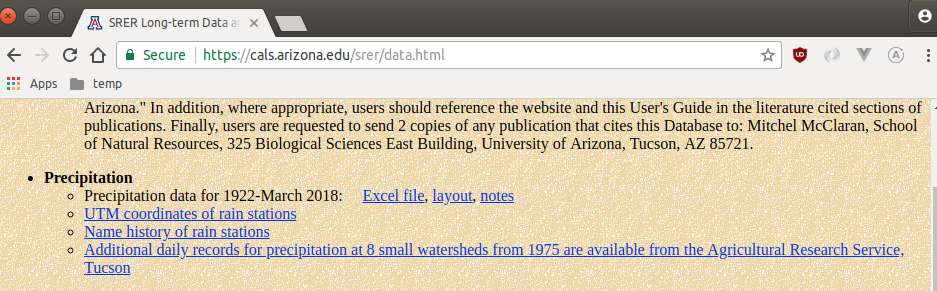
\includegraphics[width=\columnwidth]{./images/srer_precip_data_page.png}
  \caption{SRER Precipitation Data Page \cite{hid505SrerWebSite2018}}\label{f:srer_precip_data_page}
\end{figure}

\section{Data Loading}
The data sets downloaded for this demonstration were the raingage (Universal 
Transverse Mercator (UTM) coordinate data files and the Excel file that 
contained all of the preciption data for the respective raingages.  Some of 
the raingage data had to be cleaned mostly due to typographical errors and the 
UTM coordinates had to be converated to latitude and longitude values in case 
the data are rendered in mapping applications.

The precipitation data had to be converted from an Excel file to a CSV file 
and the value delimiter was changed from a comma to the pipe symbol.  The 
reason for this is because the comma can occur in some of the descriptive text 
data for raingages, where as the pipe symbol is typically not used in written 
English.

\section{Web API Development}
After the data were prepared for import into a database, the foundation for a simple web API 
application was established using the following software:

\begin{enumerate}
  \item Docker - a container platform \cite{hid505Docker2018}
  \item Python - the programming language
  \item Graphene - a Python programming language library that is used to 
  develop GraphQL APIs
  \item PostgresQL - the database server
  \item Django - a Python based model-view-controller (MVC) web development 
  framework
  \item Django Rest Framework - a Django plugin that facilitates the 
  development of REST APIs
  \item Graphene Django - a Django plugin that facilitates development of 
  GraphQL APIs
\end{enumerate}

The project source code is currently hosted at: https://github.com/acatejr/eapi.git

\subsection{REST/Swagger API}
Generally, a REST based API endpoints, in combination with a tool like Swagger 
are combined to create a web interface like the one shown in 
figure~\ref{f:rest_swagger_ui}.  The figure provides an example of the various 
API endpoints (e.g., /api/srer/v1.0/precipevents).  Some endpoints require 
input parameters which are used to execute parameterized queries (e.g. queries 
that filter data) data, while other endpoints require no parameters and 
typically return a list of data entities.

\begin{figure}[htb]
  \centering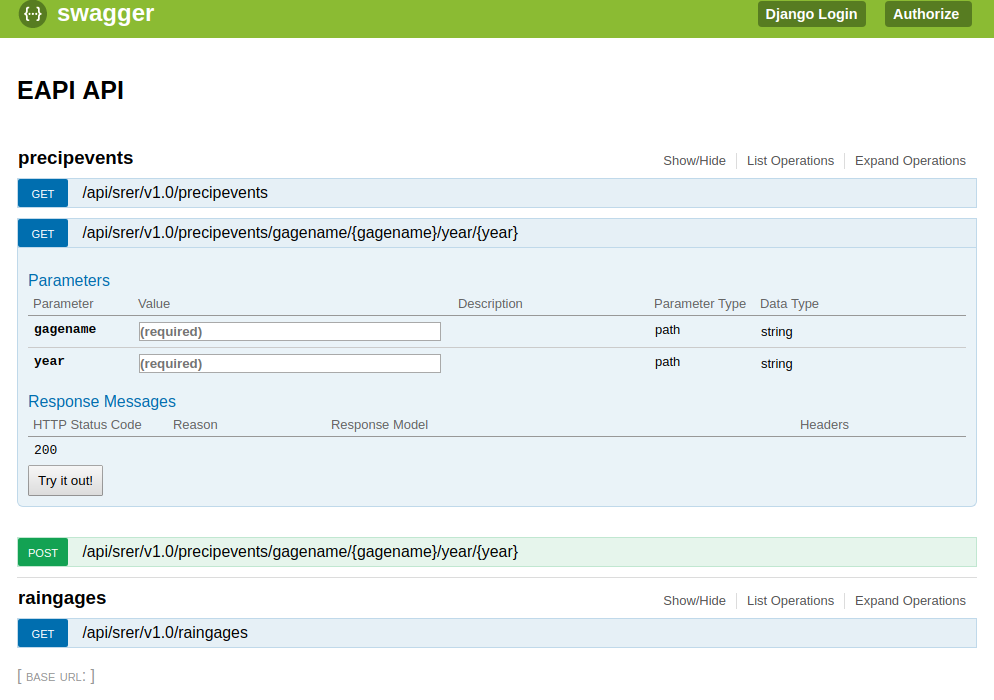
\includegraphics[width=\columnwidth]{./images/rest_swagger_ui.png}
  \caption{REST/SWAGGER UI \cite{hid505SrerWebSite2018}}\label{f:rest_swagger_ui}
\end{figure}

\subsection{GraphQL API}
Content on GraphQL here.

\section{Service Comparison}
GraphQL and REST Swagger Comparison
Describe the tools used and the development of the load testing tools.  
Also, describe the results.  Table summary, etc.

\section{Amazon Lambda}
If there is time describe and implement the Amazon Lambda that the web 
API/application can use.

\section{Raspberry Pi Cluster}
If there is time, describe and develop a three-node Raspberry Pi cluster and 
deploy the web api application to that cluser.

\section{Conclusion}
The conclusion will go here.

\begin{acks}
The authors would like to thank Dr.~Gregor~von~Laszewski for his support 
and suggestions to write this paper.
\end{acks}

\bibliographystyle{ACM-Reference-Format}
\bibliography{report} 
